\section {Frontend - Android Client}
The following section will describe the product the front-end team developed during the course.
The product consists of two different applications: Elephant, the web browser, and an implementation
of the NetInf services that support Information-Centric Networking.

\subsection{Elephant Web Browser}
The web browser application is a simple implementation

\subsection{NetInf Service}

\begin{table}
\centering
 \begin{tabular}{|c|p{10cm}|}\hline
  Functionality	& Description \\\hline
  Search	& The application searches for the hash value of the content requested, specified by a URL. This search includes
		  searching for the hash value within the local database and the remote Name Resolution Service (NRS).
		  It returns the value, if found.\\\hline
  Get		& A Get request hat contains the hash value of an Information Object (IO) triggers a content retrieval of the
		  corresponding content. The application tries to retrieve the content either from the Local Resolution Service (LRS), the NRS
		  or from a remote Bluetooth device.\\\hline
  Publish	& The services can register the local device as a locator for a content specified by a hash in the NRS. This way, remote
		  devices can try to retrieve that content from the local device using Bluetooth. \\\hline
  Full put	& The full put is a publish request that contains the actual content corresponding to the content that is published. Thus,
		  the NRS, to which the local device is connected to, can store the content and serve it itself.\\\hline
		  
 \end{tabular}
  \caption{Functionalities}\label{tab:netinffunctionalities}
\end{table}

The NetInf Services are a stand-alone application that can be used by other
applications in order to make use of Information-Centric Networking. All functionalities
that are provided are listed in \tab{netinffunctionalities}. If an application
needs our services, the NetInf Service application has to run in background.

\begin{figure}
\centering
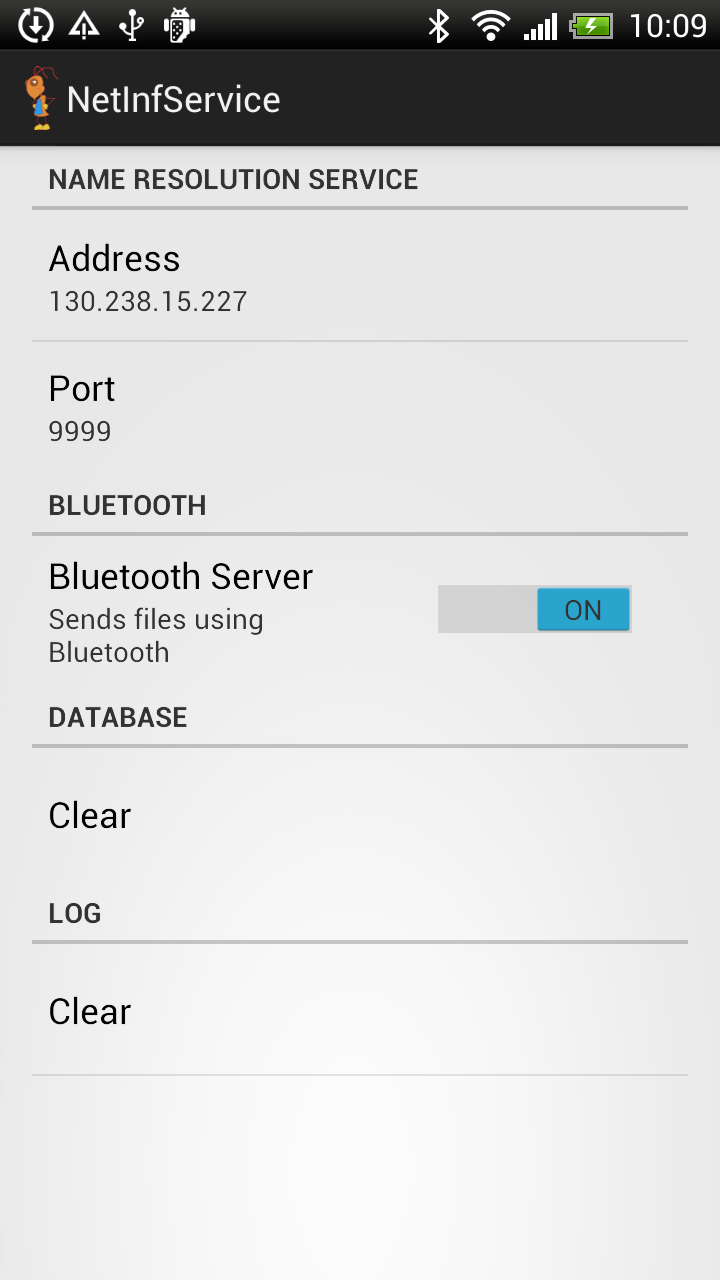
\includegraphics[scale=0.15]{img/ant_settings.png}
\caption{NetInf Service Settings}\label{fig:servicesettings}
\end{figure}

The services are configurable within a simple and self-explanatory user interface that is shown in \fig{servicesettings}.
If a user wants to change the NRS her device is communicating with,the address as well as the port can be changed accordingly.
In addition a user can decide whether she wants to share her downloaded content with another remote device. Only if the \textit{Bluetooth Server} 
is turned on, data will be shared. Else, the local device will not serve as a locator.
Finally, the database as well as the logs created during the run can be cleared.
The database stores every single content that is published. In the long run it will improve the runtime if you clear the database from
time to time, so that searches can be processed faster.
Log files are used for debugging purposes. In case a log is old, clear it and rerun the application in order to 
gain new logs.





